% This tex file is available under a
% Creative Commons Attribution-Share Alike license (CC BY-SA 2.0).
% http://creativecommons.org/licenses/by-sa/2.0/
% Copyright © 2013 Rodrigo Hausen
\documentclass{beamer}
\usepackage[utf8]{inputenc}
\usepackage{lmodern}
\usepackage[T1]{fontenc}
\usepackage[portuguese,brazil]{babel}
\usepackage{url}
\usepackage{listings}
\usepackage{color}
\usepackage{textcomp}
\usepackage{pdfpages}
\usepackage{fancyvrb}
\usepackage{enumerate}
\usepackage{alltt}
\usepackage{array}
\usepackage{slashbox}
%\usepackage[pdf]{pstricks}
%\usepackage{auto-pst-pdf}
%\usepackage{icomma} % para vírgula decimal / decimal comma
\definecolor{listinggray}{gray}{0.9}
\definecolor{mediumgray}{rgb}{0.6,0.6,0.6}
\definecolor{lbcolor}{rgb}{0.9,0.9,0.9}
\lstset{
    backgroundcolor=\color{lbcolor},
    tabsize=4,
    rulecolor=,
    basicstyle=\scriptsize,
    upquote=true,
    aboveskip={1.5\baselineskip},
    columns=fixed,
    showstringspaces=false,
    extendedchars=true,
    breaklines=true,
    prebreak = \raisebox{0ex}[0ex][0ex]{\ensuremath{\hookleftarrow}},
    frame=single,
    showtabs=false,
    showspaces=false,
    showstringspaces=false,
    identifierstyle=\ttfamily,
    keywordstyle=\color[rgb]{0,0,1},
    commentstyle=\color[rgb]{0.133,0.545,0.133},
    stringstyle=\color[rgb]{0.627,0.126,0.941},
}
\definecolor{pinegreen}{RGB}{0,139,114}
\definecolor{pgr}{RGB}{0,139,114}

\definecolor{aquamarine}{RGB}{0,181,190}
\definecolor{aqm}{RGB}{0,181,190}

\definecolor{skyblue}{RGB}{100,227,251}
\definecolor{skb}{RGB}{100,227,251}

\definecolor{pnk}{RGB}{255,150,150}

\newcommand{\comment}[1]{{\color{structure.fg!70!white}\footnotesize #1}}

\newcommand{\WD}[1]{\fbox{#1}\hspace{-0.5pt}}
\newcommand{\FWD}[1]{%
\fbox{%
\vbox to 10pt{\vfil%
\hbox to 0.8cm{\hfill#1\hfill}%
\vfil}%
}\hspace{-0.5pt}%
}

\def\A{\texttt{A}}
\def\B{\texttt{B}}
\def\C{\texttt{C}}
\def\D{\texttt{D}}
\def\E{\texttt{E}}
\def\F{\texttt{F}}

\usetheme{Boadilla}
%\usetheme{umbc2}
\usefonttheme{structuresmallcapsserif}
\usecolortheme{seahorse}

\title{Aula 11: Blocos Digitais Básicos -- Decodificador e Multiplexador}
\subtitle{Circuitos Digitais}
\author{Rodrigo Hausen}
\institute{CMCC -- UFABC} 
\date{4 e 6 de março de 2013}

\newcommand{\Not}[1]{\overline{#1}}
\def\And{\,}

\begin{document}

\begin{frame}
\maketitle

\vspace{-1cm}

\begin{center}
\url{http://compscinet.org/circuitos}
\end{center}

\end{frame}

%%%%%%%%%%%%%%%%%%%%%%%%%%%%%%%%%%%%%%%%%%%%%%%%%

\begin{frame}
\frametitle{Decodificador binário básico}

\begin{itemize}
\item \textbf{Exercício 1}: Projete um circuito digital com $4$ entradas:
$a_3, a_2, a_1, a_0$ e uma saída $X$, tal que $X = 1$ somente se $(a_3  a_2  a_1 a_0)_2 = (1001)_2$.
\end{itemize}

\pause
$$X = a_3 \; \Not{a_2} \; \Not{a_1} \; a_0$$

\pause
\begin{center}
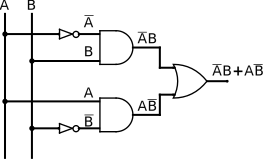
\includegraphics{images/exemplo1}
\end{center}

\end{frame}

%%%%%%%%%%%%%%%%%%%%%%%%%%%%%%%%%%%%%%%%%%%%%%%%%
\begin{frame}
\frametitle{Decodificador binário básico}

\begin{itemize}
\item \textbf{Exercício 2}: Projete um circuito digital com $4$ entradas:
$a_3, a_2, a_1, a_0$ e uma saída $X$, tal que $X = 0$ somente se $(a_3  a_2  a_1 a_0)_2 = (1001)_2$. Use apenas portas NAND.
\end{itemize}


\pause
$$X = \Not{a_3 \; \Not{a_2} \; \Not{a_1} \; a_0}$$

\pause

\begin{center}
\only<1-3>{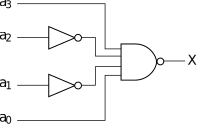
\includegraphics{images/exemplo2-0}}%
\only<4->{\includegraphics{images/exemplo2}}%
\end{center}

\end{frame}

%%%%%%%%%%%%%%%%%%%%%%%%%%%%%%%%%%%%%%%%%%%%%%%%%
\begin{frame}
\frametitle{Decodificador binário básico}

\begin{itemize}
\item \textbf{Decodificador básico:} identifica um código binário na entrada.
\pause
\item Os exemplos abaixo identificam o código $(1001)_2 = (9)_{10}$
\end{itemize}

\vspace{12pt}

\begin{minipage}{0.47\textwidth}
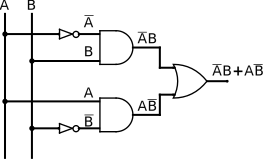
\includegraphics{images/exemplo1}\\
saída em nível \textbf{alto}
\end{minipage}\pause
\hfill
\begin{minipage}{0.47\textwidth}
\includegraphics{images/exemplo2}\\
saída em nível \textbf{baixo}
\end{minipage}
\end{frame}

%%%%%%%%%%%%%%%%%%%%%%%%%%%%%%%%%%%%%%%%%%%%%%%%%
\begin{frame}
\frametitle{Decodificador binário}

\begin{itemize}
\item \textbf{Exercício 3}: faça um circuito com quatro entradas $a_3, a_2, a_1,
a_0$ e três saídas $X_5, X_9$ e $X_{13}$ tais que cada uma delas identifique
a entrada dos números $5$, $9$ e $13$, respectivamente, por meio de um
sinal de nível \textbf{alto}.
\end{itemize}

\pause

$X_5 = \Not{a_3} \; a_2 \; \Not{a_1} \; a_0$ \hfill 
$X_9 = a_3 \; \Not{a_2} \; \Not{a_1} \; a_0$ \hfill
$X_{13} = a_3 \; a_2 \; \Not{a_1} \; a_0$

\pause

\begin{center}

\includegraphics{images/exemplo3}
\end{center}

\end{frame}

%%%%%%%%%%%%%%%%%%%%%%%%%%%%%%%%%%%%%%%%%%%%%%%%%
\begin{frame}[fragile]
\frametitle{Decodificador binário}

\begin{itemize}
\item \textbf{Exercício 4}: faça um circuito com quatro entradas $a_3, a_2, a_1,
a_0$ e $16$ saídas $X_0, X_1, X_2, \ldots, X_{15}$ tais que cada uma delas
identifique a entrada do número $0$, $1$, $2$, \ldots, $15$, respectivamente,
por meio de um sinal de nível \textbf{alto}.
\end{itemize}

\pause

\begin{eqnarray*}
X_0    & = & \Not{a_3} \; \Not{a_2} \; \Not{a_1} \; \Not{a_0} \\
X_1    & = & \Not{a_3} \; \Not{a_2} \; \Not{a_1} \; a_0 \\
X_2    & = & \Not{a_3} \; \Not{a_2} \; a_1 \; \Not{a_0} \\
X_3    & = & \Not{a_3} \; \Not{a_2} \; a_1 \; a_0 \\
        & \vdots & \\
X_{15} & = & a_3 \; a_2 \; a_1 \; a_0
\end{eqnarray*}

\pause

$4$ portas NOT, $16$ portas AND com quatro entradas

\end{frame}

%%%%%%%%%%%%%%%%%%%%%%%%%%%%%%%%%%%%%%%%%%%%%%%%%
\begin{frame}
\frametitle{Decodificador binário}

\textbf{Decodificador $n$ entradas para $2^n$ saídas:} circuito digital
com:
\begin{itemize}
\item $n$ entradas: $a_{n-1}, a_{n-2}, \ldots a_1, a_0$
\item $2^n$ saídas: $X_0, X_1, \ldots, X_{2^n-1}$
\end{itemize}
Onde a saída $X_i$ está ativa se o código $i = (a_{n-1} a_{n-2} \ldots a_1 a_0)_2$ está na entrada.

\pause
\centering
\begin{minipage}{44mm}
\only<1-2>{\includegraphics{images/decod_high}}
\only<3>{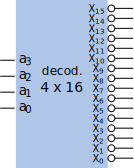
\includegraphics{images/decod_low}}
\end{minipage}
\begin{minipage}{50mm}
Decodificador $4$ para $16$\\
com saída ativa em nível
\only<1-2>{\textbf{alto}}
\only<3>{\textbf{baixo}}
\end{minipage}

\end{frame}

%%%%%%%%%%%%%%%%%%%%%%%%%%%%%%%%%%%%%%%%%%%%%%%%%
\begin{frame}
\frametitle{Decodificador binário: aplicação}

\begin{itemize}
\item \textbf{Pisca-pisca de natal} (sequencial de luzes) com um
decodificador e um contador binários.
\end{itemize}

\begin{center}
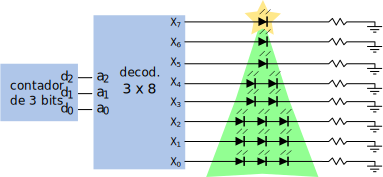
\includegraphics{images/sequencial}
\end{center}

Ver circuito \url{circuits/app_decoder.circ}

\end{frame}

%%%%%%%%%%%%%%%%%%%%%%%%%%%%%%%%%%%%%%%%%%%%%%%%%
\begin{frame}
\frametitle{Codificador Binário (Encoder)}

\textbf{Codificador $2^n$ para $n$:} Faz a operação reversa do codificador. 
\begin{itemize}
\item $2^n$ entradas: $X_0, X_1, \ldots, X_{2^n-1}$
\item $n$ saídas: $a_{n-1}, a_{n-2}, \ldots a_1, a_0$
\end{itemize}

\vspace{6pt}

\pause
\begin{center}
\begin{minipage}{44mm}
\only<1-2>{\includegraphics{images/encod_high}}
\only<3->{\includegraphics{images/encod_low}}
\end{minipage}
\begin{minipage}{50mm}
Codificador $16$ para $4$\\
com entrada ativa em nível
\only<1-2>{\textbf{alto}}
\only<3->{\textbf{baixo}}
\end{minipage}
\end{center}

\vspace{6pt}

\pause\pause

{\small
\textbf{Para casa:} fazer os diagramas dos codificadores $2$ para $1$,
$4$ para $2$ e $8$ para $3$ com
entradas: (a) ativas em nível alto; (b) ativas em nível baixo.}

\end{frame}

%%%%%%%%%%%%%%%%%%%%%%%%%%%%%%%%%%%%%%%%%%%%%%%%%
\begin{frame}
\frametitle{Multiplexador}

\textbf{Exercício 5:} Faça um circuito com:
\begin{itemize}
\item três entradas: $D_0, D_1, S_0$
\item uma saída: $Y$
\end{itemize}
tal que $Y = D_i$ se $S_0 = i$.

\pause
\vspace{6pt}

Tabela verdade:

\def\F{\fbox}

\begin{minipage}{0.3\textwidth}
\begin{tabular}{ccc||c}
$D_0$ & $D_1$ & $S_0$ & $Y$ \\
\hline
\F0  &    0   &   0   &  0  \\
  0  &  \F0   &   1   &  0  \\
\F0  &    1   &   0   &  0  \\
  0  &  \F1   &   1   &  1  \\
\F1  &    0   &   0   &  1  \\
  1  &  \F0   &   1   &  0  \\
\F1  &    1   &   0   &  1  \\
  1  &  \F1   &   1   &  1
\end{tabular}
\end{minipage}
\hfill \pause
\begin{minipage}{0.65\textwidth}
$Y = \Not{S_0} D_0 + S_0 D_1$\\[6pt]
\pause

\includegraphics{images/exercicio5}
\end{minipage}

\end{frame}

%%%%%%%%%%%%%%%%%%%%%%%%%%%%%%%%%%%%%%%%%%%%%%%%%
\begin{frame}
\frametitle{Multiplexador}

\textbf{Exercício 6:} Faça um circuito com:
\begin{itemize}
\item seis entradas: $D_0, D_1, D_2, D_3, S_0, S_1$
\item uma saída: $Y$
\end{itemize}
tal que $Y = D_i$ se $(S_1 S_0)_2 = i$.

\pause
\vspace{6pt}

``Tabela verdade'':\\[6pt]

\def\F{\fbox}

\begin{minipage}{0.3\textwidth}
\begin{tabular}{cc||c}
$S_1$ & $S_0$ & $Y$ \\
\hline
  0   &   0   & $D_0$ \\
  0   &   1   & $D_1$ \\
  1   &   0   & $D_2$ \\
  1   &   1   & $D_3$
\end{tabular}
\end{minipage}

\uncover<3>{
\vspace{6pt}
$Y = \Not{S_1} \; \Not{S_0} \, D_0 +
     \Not{S_1} \,      S_0  \, D_1 +
          S_1  \, \Not{S_0} \, D_2 +
          S_1  \,      S_0  \, D_3$
}

\end{frame}

%%%%%%%%%%%%%%%%%%%%%%%%%%%%%%%%%%%%%%%%%%%%%%%%%
\begin{frame}
\frametitle{Multiplexador}

\comment{Exercício 6 -- continuação}\\[6pt]

$Y = \Not{S_1} \; \Not{S_0} \, D_0 +
     \Not{S_1} \,      S_0  \, D_1 +
          S_1  \, \Not{S_0} \, D_2 +
          S_1  \,      S_0  \, D_3$

\only<1>{\vspace*{58mm}}%
\only<2>{\includegraphics{images/mux4x1_0}}%
\only<3>{\includegraphics{images/mux4x1_1}}%
\only<4>{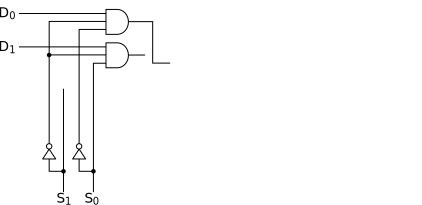
\includegraphics{images/mux4x1_2}}%
\only<5>{\includegraphics{images/mux4x1_3}}%
\only<6>{\includegraphics{images/mux4x1_4}}%
\only<7>{\includegraphics{images/mux4x1_5}}%
\only<8>{\includegraphics{images/mux4x1_6}}%
\only<9>{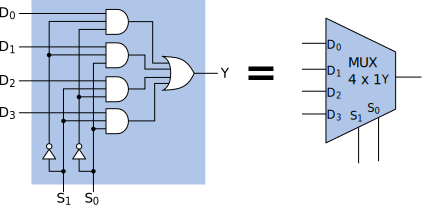
\includegraphics{images/mux4x1_7}}%
\only<10>{\includegraphics{images/mux4x1}}%

\end{frame}

%%%%%%%%%%%%%%%%%%%%%%%%%%%%%%%%%%%%%%%%%%%%%%%%%
\begin{frame}
\frametitle{Multiplexador}

Outra maneira de se construir um MUX $4\times1$

\begin{center}
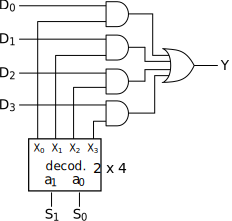
\includegraphics{images/mux4x1_decod}
\end{center}
\end{frame}

%%%%%%%%%%%%%%%%%%%%%%%%%%%%%%%%%%%%%%%%%%%%%%%%%
\begin{frame}
\frametitle{Multiplexador}

\begin{itemize}
\item Um \textbf{multiplexador} (ou MUX) $2^k \times 1$ é um circuito
com:
\begin{itemize}
\item $k$ entradas de seleção de dado: $S_0, S_1, \ldots, S_{k-1}$\\
(também chamadas entradas de endereço)
\pause
\item $2^k$ entradas de dado: $D_0, D_1, \ldots, D_{2^k-1}$
\pause
\item uma saída: $Y = D_i$ se $i = (S_{k-1} S_{k-2} \ldots S_1 S_0)_2$
\end{itemize}
\end{itemize}
\pause
\begin{center}
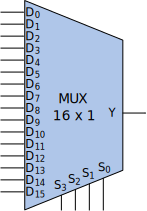
\includegraphics[scale=0.9]{images/mux16x1}
\end{center}
\end{frame}

%%%%%%%%%%%%%%%%%%%%%%%%%%%%%%%%%%%%%%%%%%%%%%%%%
\begin{frame}
\frametitle{Multiplexador}

\textbf{Exercício 7:} Construa um MUX $8\times1$ a partir de multiplexadores menores.
\begin{itemize}
\item Endereço: $S_2, S_1, S_0$; \hspace{2ex} Dados: $D_0, D_1, \ldots, D_7$
\end{itemize}

\pause

\begin{center}
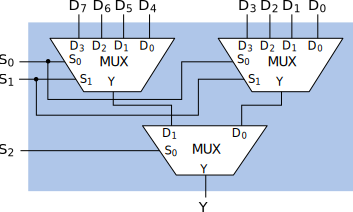
\includegraphics{images/mux8x1_composite}
\end{center}

\end{frame}

%%%%%%%%%%%%%%%%%%%%%%%%%%%%%%%%%%%%%%%%%%%%%%%%%
\begin{frame}
\frametitle{Multiplexador}

\textbf{Para casa:}\\
(a) Construa um MUX $16\times1$ com multiplexadores $4\times1$.\\
(b) Construa um MUX $16\times1$ com multiplexadores $2\times1$.

\end{frame}

%%%%%%%%%%%%%%%%%%%%%%%%%%%%%%%%%%%%%%%%%%%%%%%%%
\begin{frame}
\frametitle{Multiplexador: aplicação}

\begin{itemize}
\item \textbf{Exercício 8}: construa um circuito com:
\begin{itemize}
\item $8$ entradas de dados $b_3, b_2, b_1, b_0$, $a_3, a_2, a_1, a_0$
\item $1$ entrada de seleção $Op$
\item $4$ saídas $s_3, s_2, s_1, s_0$
\end{itemize}
tal que $$
(s_3 s_2 s_1 s_0)_2 = \left\{
\begin{array}{ll}
(b_3 b_2 b_1 b_0)_2 + (a_3 a_2 a_1 a_0)_2 & \text{se } Op = 0 \\
(b_3 b_2 b_1 b_0)_2 - (a_3 a_2 a_1 a_0)_2 & \text{se } Op = 1 \\
\end{array}
\right.
$$
\end{itemize}
Todas as operações são com números sem sinal. Desconsidere os casos em que há overflow.
\end{frame}


%%%%%%%%%%%%%%%%%%%%%%%%%%%%%%%%%%%%%%%%%%%%%%%%%
\begin{frame}
\frametitle{Resposta exercício 8}

\only<1>{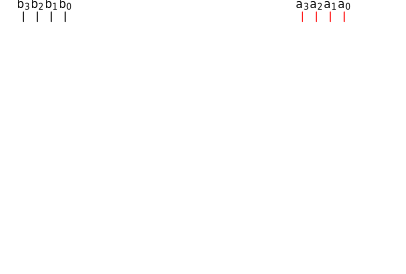
\includegraphics{images/ula1_0}}%
\only<2>{\includegraphics{images/ula1_1}}%
\only<3>{\includegraphics{images/ula1_2}}%
\only<4>{\includegraphics{images/ula1_3}}%
\only<5>{\includegraphics{images/ula1_4}}%
\only<6>{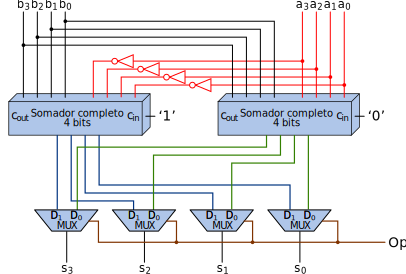
\includegraphics{images/ula1_5}}%
\only<7>{\includegraphics{images/ula1}}%

\end{frame}

%(Solução na lousa)
%
%\pause
%
%\vspace{12pt}
%
%Este circuito é chamado Unidade Lógico-Aritmética (ULA ou ALU) de
%$4$ bits.
%Esta ULA faz apenas as operações de soma $A+B$ e subtração $A-B$.
%\end{frame}

%%%%%%%%%%%%%%%%%%%%%%%%%%%%%%%%%%%%%%%%%%%%%%%%%
\begin{frame}
\frametitle{Unidade Lógico-Aritmética}

\begin{itemize}
\item \textbf{Unidade Lógico-Aritmética (ULA)}: circuito digital
que faz operações lógicas e aritméticas. A operação a ser
feita é selecionada pelos bits de seleção de operação
$Op_0, Op_1, \ldots$.
\begin{itemize}
\item A ULA do exercício anterior só possui $1$ bit de operação,
para escolher entre soma e subtração.
\end{itemize}
\end{itemize}

\pause

\begin{itemize}
\item \textbf{Para casa}: construa um circuito com:
\begin{itemize}
\item $8$ entradas de dados $b_3, b_2, b_1, b_0$, $a_3, a_2, a_1, a_0$
\item $2$ entradas de seleção $Op_1, Op_0$
\item $4$ saídas $s_3, s_2, s_1, s_0$
\end{itemize}
tal que $$
(s_3 s_2 s_1 s_0)_2 = \left\{
\begin{array}{ll}
(b_3 b_2 b_1 b_0)_2 + (a_3 a_2 a_1 a_0)_2 & \text{se } (Op_1 Op_0)_2 = 0 \\
(b_3 b_2 b_1 b_0)_2 - (a_3 a_2 a_1 a_0)_2 & \text{se } (Op_1 Op_0)_2 = 1 \\
(a_3 a_2 a_1 a_0)_2 + 1 & \text{se } (Op_1 Op_0)_2 = 2 \\
(a_3 a_2 a_1 a_0)_2 - 1 & \text{se } (Op_1 Op_0)_2 = 3 \\
\end{array}
\right.
$$
\end{itemize}
Todas as operações são com números sem sinal. Desconsidere os casos em que há overflow.

\end{frame}


%%%%%%%%%%%%%%%%%%%%%%%%%%%%%%%%%%%%%%%%%%%%%%%%%
\begin{frame}
\frametitle{Demultiplexador}

\textbf{Demultiplexador} (DEMUX): faz a operação reversa do multiplexador.

\begin{center}
\begin{minipage}{0.4\textwidth}
\includegraphics{images/demux1x16}
\end{minipage}
\hspace{0.1\textwidth}
\pause
\begin{minipage}{0.4\textwidth}
\textbf{Para casa:} fazer os circuitos para os
demultiplexadores\\ $1 \times 2$, $1 \times 4$,
$1 \times 8$ e $1 \times 16$

\vspace{12pt}
\textbf{Dica:} use decodificadores.
\end{minipage}
\end{center}

\end{frame}

%%%%%%%%%%%%%%%%%%%%%%%%%%%%%%%%%%%%%%%%%%%%%%%%%
\begin{frame}
\frametitle{Para casa}

\begin{itemize}
\item Ler seções 6-5, 6-6, 6-8 e 6-9
\begin{itemize}
\item Lembre-se: Leia e entenda! Não decore! Decorar funcionamento e
descrição de circuito integrado não vale a pena!
\end{itemize}
\item Ler seções 6-7 e 6-10 para aumentar a sua cultura.
\item Exercícios: autotestes 7, 10, 11; problemas 14--18, 26, 27.
\item \textbf{Importante:} lembre-se de fazer também os outros
problemas para casa nestes slides.
\end{itemize}
\end{frame}

\end{document}
